\documentclass[thesis.tex]{subfiles}
\begin{document}

\chapter{Introduction}
\label{chap:introduction}

% An image right here at the top can look really cool!

\section{Introduction}
The current Internet has exceeded any expectations. The engineers creating it in the 1960s couldn't even imagine the impact and various use of their creation. Only few users participated in the early Internet without considering security and protection against attacks as a key aspect. There were so few people that they knew who they can trust and who not.

Today there are billions of users and devices connected to each other \cite{MiniwattsMarketingGroup.31.12.2017}. Unfortunately, there are also malicious user trying to disturb the network by overusing resources or manipulation the members. More and more services are created each year running on the Internet and trying to provide a service to users. Each company has to know the newest security risks and attack types to be competitive and trustworthy. 

There are many types of problems with the current Internet protocols. There are far more fixes and solutions with them, but each of them has to be accepted by the majority of the users and supported by the network device manufacturers. The acceptance of IPv6, a protocol released in 1996, is low in 2017 but the Internet ran out of IPv4 addresses in 2011 \cite{ICANN.03.02.2011}.

Instead of fixing the current Internet and trying to patch the structural problems from past designs, there are also people creating a better green field solution. They want to solve the problems without limitations of the current protocols and their implicit fundamental problems. One of the solutions is \textbf{SCION}, that stands for \textbf{S}calability, \textbf{C}ontrol and \textbf{I}solation \textbf{O}n next-generation \textbf{N}etworks, which will be explained in detail in \autoref{chap:basics}.


\section{Motivation}
One of the many issues is the strong increase of traffic on the Internet. The DE-CIX in Frankfurt, Germany, a data carrier, accounts each year a higher amount of data as shown in \autoref{fig:intro:decixData}. In 2014 the peak was around three TB/s. Three years later in 2017 the peak was at 6 TB/s, i.e. twice the amount. 

In the advent of video streaming in form of Video on Demand (VOD) via services like YouTube\footnote{\url{https://www.youtube.com}, 20.04.2018} and Netflix\footnote{\url{https://www.netflix.com}, 20.04.2018} and live video streaming like Twitch\footnote{\url{https://www.twitch.tv/}, 20.04.2018} the data usage of the users increased rapidly. There is also an increasing demand for higher resolutions, which results in bigger video sizes. The current standard of Full HD for a video will be succeeded by new standards like the 4K. The user also demands for a higher frame rate. Currently, the videos are sent with 30fps, but there is a benefit using 60fps or even 144fps for really fast movements.

But videos are not the only reason for a higher bandwidth usage. Big Data companies processing petabytes of data each day rely on a stable and high bandwidth connection. There is also a trend with Internet-of-Things (IoT) to install small devices which collect and send data through the Internet.

The stability of the current Internet is also a motivation to improve the structure of it. Attacks like \textbf{D}istributed \textbf{D}enial-\textbf{o}f-\textbf{S}ervice (DDos) using the resources to disrupt the operation of companies or governments are increasing in size and frequency \cite{GoogleInc.2013}. But also technical problem like a power outage \cite{DECIX.10.04.2018} or an environmental hazard (earthquakes, floods) can disturb the stability of the Internet when a central node fails. 

\begin{figure}
    \centering
    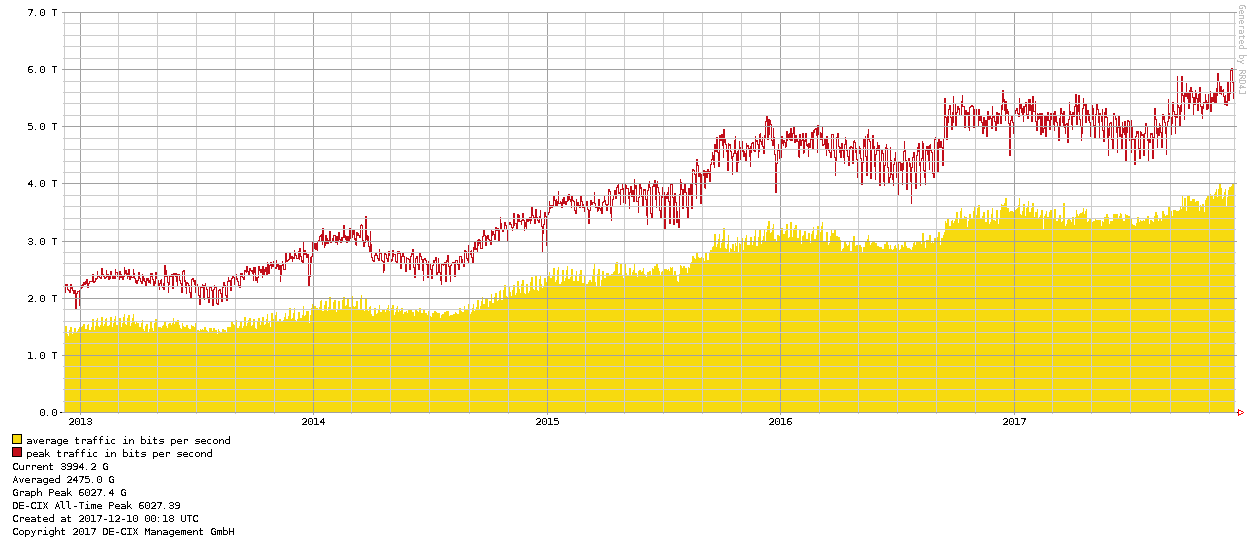
\includegraphics[width=0.95\linewidth]{20171210_1515_decix_data}
    \caption*{\tiny{ \url{https://www.de-cix.net/en/locations/germany/frankfurt/statistics} (10.12.2017)}}
    \caption{5-year graph of the average exchanged traffic at DE-CIX in Frankfurt, Germany}
    \label{fig:intro:decixData}
\end{figure}

One solution to solve this problems is to scale-up and install more and more bandwidth capacities like fiber cables or newer devices. This is inefficient and consumes probably more energy and thus increases the running costs. There are also physical limits for improving the performance so that a small benefit results in high costs.

Another solution is to better utilize the current resources as it is done with the multi-path feature in SCION. Here the users can split their data and sent the packets via multiple connections. This leads to a better usage of the available bandwidth in the network. In the current Internet this is not possible, because the router are deciding for themselves which route to take to the destination. 

\begin{figure}[h]
    \centering
    \begin{tikzpicture}
    \node[shape=rectangle,draw=black] (1-1) at (0,0) {1-1};
    \node[shape=rectangle,draw=black] (1-2) at (2,-1) {1-2};
    \node[shape=rectangle,draw=black] (1-3) at (2,1) {1-3};
    \node[shape=rectangle,draw=black] (1-4) at (4,0) {1-4};
    
    \path[-]	
    (1-1) edge node[sloped, anchor=center, below] {\tiny 1GB/s} (1-2) 
    (1-1) edge node[sloped, anchor=center, above] {\tiny 1GB/s} (1-3)
    (1-1) edge node[sloped, anchor=center, above] {\tiny 1GB/s} (1-4)
    (1-2) edge node[sloped, anchor=center, below] {\tiny 1GB/s} (1-4)
    (1-3) edge node[sloped, anchor=center, above] {\tiny 1GB/s} (1-4)
    ;
    \path[-{Latex[width=3mm]}, dashed]
    (1-1) edge[bend right=10] (1-4)
    (1-1) edge[bend left=80] (1-4)
    (1-1) edge[bend right=80] (1-4)
    ;
    \end{tikzpicture}
    \caption{Example topology for multipath}
    \label{fig:intro:exampleMultipath}
\end{figure}


This new method shall encourages user to better utilize the network, but it can also be misused. In \autoref{fig:intro:exampleMultipath} an example is visualized. Each AS, but not 1-2 to 1-3 is connected with each other via a 1 GBit/s connection. AS 1-1 can send AS 1-4 data using single path with a 1 GBit/s directly. It could also uses the paths 1-1$\rightarrow$1-2$\rightarrow$1-4 and 1-1$\rightarrow$1-3$\rightarrow$1-4 to send its data and increase its bandwidth to ideally 3 gigabit/s, if there is zero delay on the hops. This possibility rises the questions how to monitor and enforce the bandwidth usage of a one particular AS. When using a single path connection the measurement point is at the destination. If this AS exceeds its limit the destination router can drop packets. This solution is not possible in a multi-path environment. It is important to find an answer for this question to avoid misuse.

\section{Goals} \label{sec:intro:goals}

The work was planned and executed with the following described goals in mind. They will be evaluated in \autoref{chap:eva} and tested if their have been achieved by the proposed approach in this work.
     \begin{easylist}
        \MyNumberedListProperties
        # The thesis' main goal is to achieve a fair usage of bandwidth using multi-path communication in SCION. The proposed solution must not use more resources (computation time, bandwidth) than it will gain through using the bandwidth more efficiently. A solution with a 100\% accuracy is not necessary if it uses too much resources. Because of this, the goals must always reach a trade-off between efficiency (resource usage) and effect (resource gain).        
        # The first goal to verify is, that the proposed solution has to detect a greedy user as accurately as possible with the least possible performance impact.
        # The solution must also provide parameters to increase the accuracy of the detection rate, even when the performance impact will be higher. This is important for an adaption in systems who requires an higher detection.
        # It is also a goal to create a scalable solution working with topologies with a number in the order of hundreds or thousand nodes. This goal will be achieved by minimizing the impact on network traffic for necessary protocols.
        # The solution must be general enough for other network types with multi-path capability.        
        # Based on the previous goal, this thesis will provide an implementation for SCION which can be used inside SCIONLab.
    \end{easylist}

\section{Main Contribution}
The proposed contribution will provide a solution to identify user inside a network with a small impact on the networks performance. It will use a heuristic based selection algorithm to only monitor interesting nodes. This leads to a small amount of necessary nodes to receive a high enough coverage of the networks traffic to identify nodes which overuses their resources. The approach will be created for networks in general and will have an proof of work implementation for the SCIONLab network structure.

\section{Thesis Outline}
This thesis is divided into six chapters and an appendix. The first chapter \autoref{chap:introduction} introduced the problem and provided a motivation to solve such a problem. It defined goals to get achieved and outlined the main contribution to the topic.

The next chapter \autoref{chap:preqAndRel} explains the necessary requirements to understand and follow this work and related work to this topic. It explains how the SCION network is working and what the used tool, Prometheus, is. The related work will contain already existing works relating to the topic, such as SIPRA for SCION itself and results of other researcher. 

The third chapter, \autoref{chap:main} describes main contribution of this work, the SpeedCam approach based on the inspection game. It is described in a concept for networks in general and will be defined for the SCION structure. This chapter will also formulate theses and assumption of the influence of featured variables.

These will be evaluated in \autoref{chap:eva}, which contains the experiment to show the results. It will firstly describe the setup for the evaluation and will than show and discuss the results of it.

This work will be concluded in the last chapter \autoref{chap:concl}. This will summarize the work, conclude the results and give an overview of new questions and problems to solve in further works.

The appendix will contain configurations and listings to reproduce the results.

\subfilebib % Makes bibliography available when compiling as subfile
\end{document}